\documentclass[11  pt]{exam} 
\usepackage[lmargin=1in,rmargin=1.75in,bmargin=1in,tmargin=1in]{geometry}  


% For hyperlinking everything
\usepackage{hyperref}
\hypersetup{
	colorlinks=true, %set true if you want colored links
	linktoc=all,     %set to all if you want both sections and subsections linked
	linkcolor=blue,  %choose some color if you want links to stand out
}


\usepackage[latin1]{inputenc}
\usepackage{amsmath}
\usepackage{mathrsfs}  
\usepackage{amsfonts}
\usepackage{amssymb}
\usepackage{graphicx}
\usepackage{subfig}
\usepackage{caption}
\usepackage{algorithm}
%\usepackage{algcompatible}
%\usepackage{algorithmicx}
\usepackage{algpseudocode}

\usepackage{titlesec}
\titleformat{\section}{\fontfamily{lmss}\fontsize{14}{15}\bfseries}{\thesection}{1em}{}
\titleformat{\subsection}{\fontfamily{lmss}\fontsize{12}{15}\bfseries}{\thesubsection}{1em}{}




\usepackage{amsthm}

\newtheoremstyle{noit}
{10pt}% <Space above>
{10pt}% <Space below>
{}% <Body font>
{}% <Indent amount>
{\bfseries}% <Theorem head font>
{.}% <Punctuation after theorem head>
{.5em}% <Space after theorem headi>
{}% <Theorem head spec (can be left empty, meaning `normal')>

\newtheoremstyle{example}
{10pt}% <Space above>
{10pt}% <Space below>
{}% <Body font>
{20pt}% <Indent amount>
{\bfseries}% <Theorem head font>
{.}% <Punctuation after theorem head>
{.5em}% <Space after theorem headi>
{}% <Theorem head spec (can be left empty, meaning `normal')>


\newtheoremstyle{indented}{20pt}{20pt}{\addtolength{\leftskip}{2.5em}}{}{\bfseries}{.}{.5em}{}


\newtheorem{theorem}{Theorem}
\numberwithin{theorem}{section}
\newtheorem{lemma}[theorem]{Lemma}
\newtheorem{corollary}[theorem]{Corollary}
\newtheorem{observation}{Observation}
%\numberwithin{observation}{section}
%\numberwithin{definition}{section}
\newtheorem{conjecture}{Conjecture}
\newtheorem{Qu}{Question}
\newcommand{\QU}{\begin{Qu}\normalfont}

\theoremstyle{noit}
\newtheorem{fact}{Fact}
\newtheorem{definition}{Definition}

\theoremstyle{indented}
\newtheorem{example}{Example}

\theoremstyle{indented}
\newtheorem{problem}{Problem}


%\newenvironment{proof}{\noindent{\bf Proof:} \hspace*{1em}}{
%    \hspace*{\fill} $\Box$ }
%\newenvironment{proof_of}[1]{\noindent {\bf Proof of #1:}
%    \hspace*{1em} }{\hspace*{\fill} $\Box$ }
%\newenvironment{proof_claim}{\begin{quotation} \noindent}{
%    \hspace*{\fill} $\diamond$ \end{quotation}}
\newcommand{\vs}[1]{\vspace{#1}}

\newcommand{\lecture}[2]{
 \noindent
\begin{center}
	\framebox{
		\vbox{
			\hbox to 5.78in { {\bf CSCE 411: Design and Analysis of Algorithms} \hfill  }
			\vspace{2mm}
			\hbox to 5.78in { {\Large \hfill Lecture #1\hfill} }
			\vspace{2mm}
			\hbox to 5.78in { {\it Date: #2 \hfill Lecturer: Nate Veldt} }
		}
	}
\end{center}
\vspace*{4mm}
}


\newcommand{\hw}[2]{
	\noindent
	\begin{center}
		\framebox{
			\vbox{
				\hbox to 5.78in { {\bf CSCE 411: Design and Analysis of Algorithms} \hfill  }
				\vspace{2mm}
				\hbox to 5.78in { {\Large \hfill Homework #1\hfill} }
				\vspace{2mm}
				\hbox to 5.78in { {\it Due date: #2 \hfil} }
			}
		}
	\end{center}
	\vspace*{4mm}
}



\newcommand{\under}[1]{\underline{\hspace{#1}}}
\setlength{\parindent}{0em}

%\usepackage[tagged]{accessibility}

% Graph terms
\newcommand{\vol}{\textbf{vol}}
\newcommand{\cut}{\textbf{cut}}


% Matrices
\newcommand{\mA}{\textbf{A}}
\newcommand{\mB}{\textbf{B}}

% vectors
\newcommand{\ve}{\textbf{e}}
\newcommand{\vx}{\textbf{x}}


% Other
\newcommand{\calN}{\mathcal{N}}

\usepackage{mathtools}
\DeclarePairedDelimiter\ceil{\lceil}{\rceil}
\DeclarePairedDelimiter\floor{\lfloor}{\rfloor}


\newcommand*{\aitem}{ \item[{
\includegraphics[width=0.8cm,height=0.5cm]{../../Lectures/figures/A}} ]  }
\newcommand*{\bitem}{ \item[{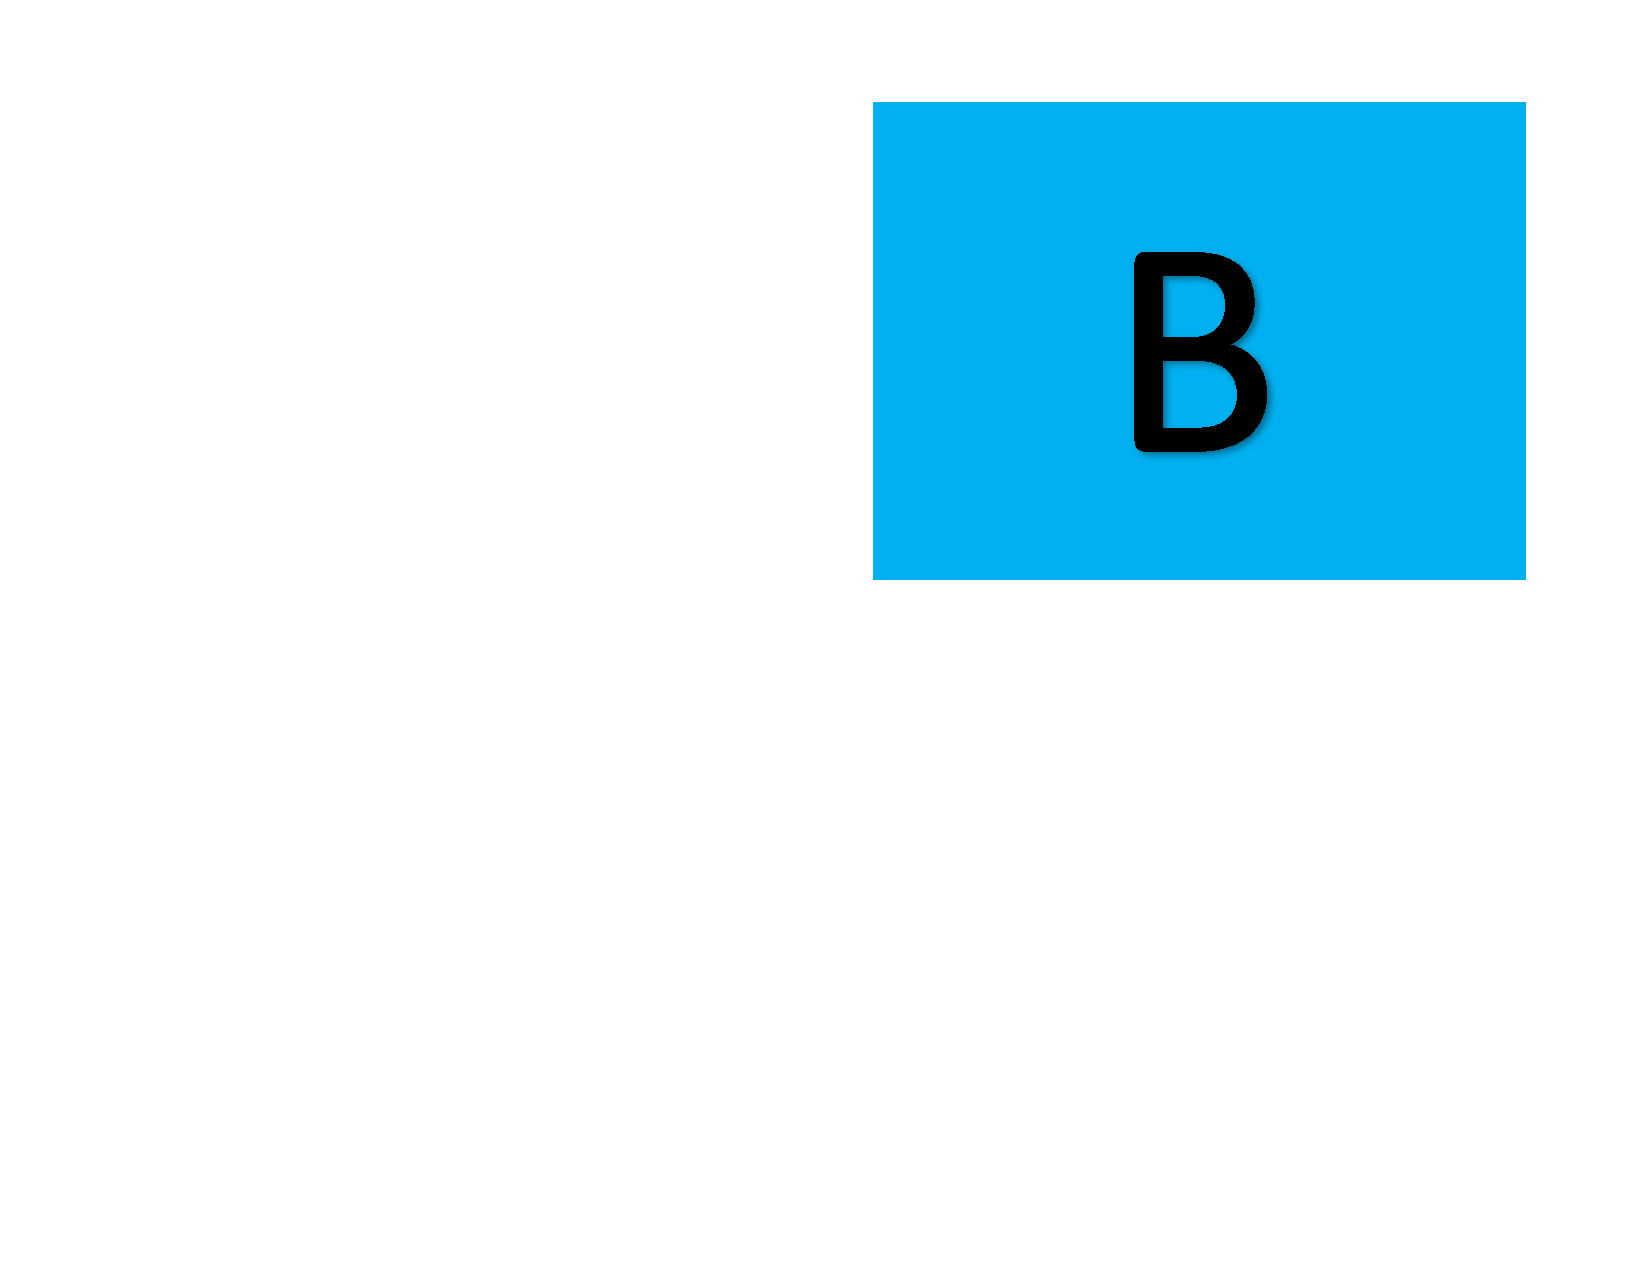
\includegraphics[width=0.8cm,height=0.5cm]{../../Lectures/figures/B}} ]  }
\newcommand*{\citem}{ \item[{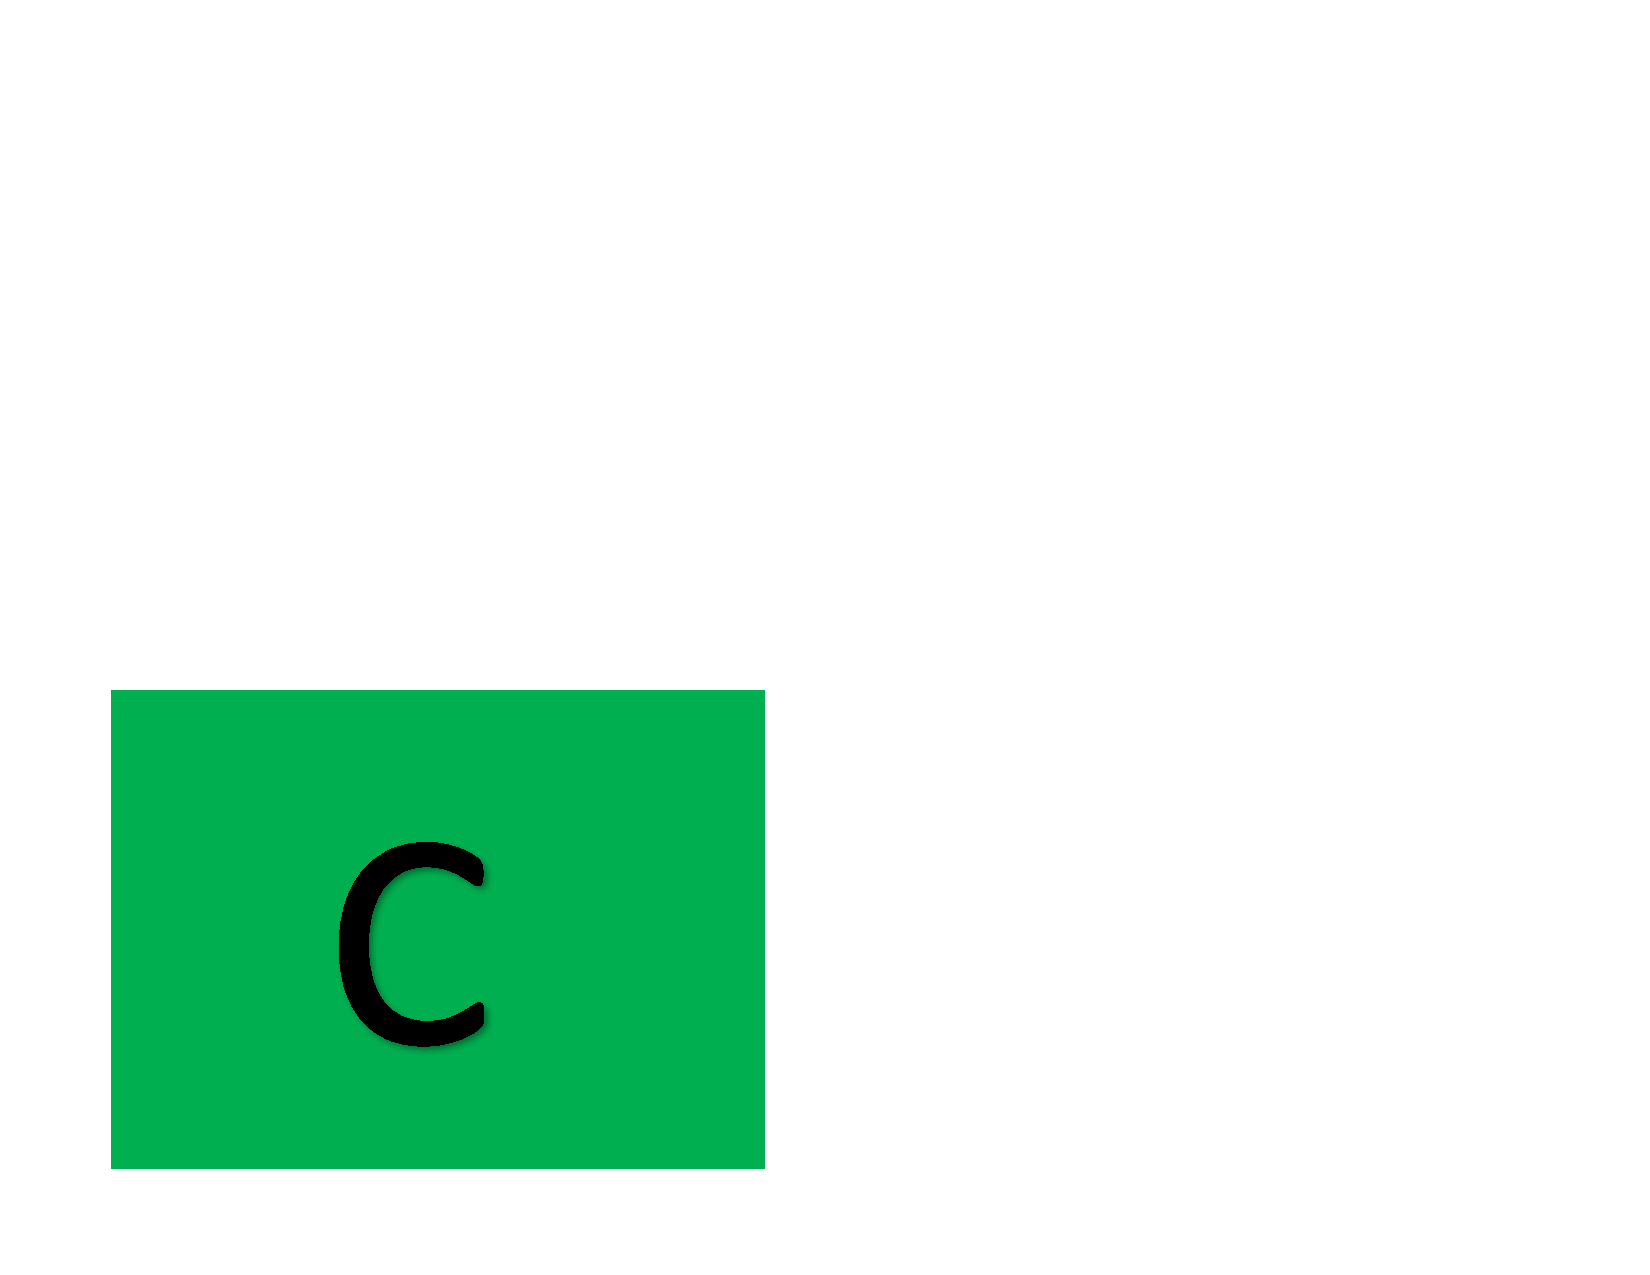
\includegraphics[width=0.8cm,height=0.5cm]{../../Lectures/figures/C}} ]  }
\newcommand*{\ditem}{ \item[{
\includegraphics[width=0.8cm,height=0.5cm]{../../Lectures/figures/D}} ]  }
\newcommand*{\eitem}{ \item[{
\includegraphics[width=0.8cm,height=0.5cm]{../../Lectures/figures/E}} ]  }
\newcommand*{\fitem}{ \item[{
\includegraphics[width=0.8cm,height=0.5cm]{../../Lectures/figures/F}} ]  }


\newcommand{\hide}[1]{\underline{\phantom{#1 #1}}}

\usepackage{setspace}

\onehalfspacing

\begin{document}
	
	
	\lecture{9: Intro to Graph Algorithms}{February 18}
	
	\section{Graph Notation and Terminology}
	
	An (undirected) graph $G = (V,E)$ is defined by  %$V = \{1, 2, \hdots, n\}$, and edges $E \subseteq V \times V$.
	\vspace{1.5cm}
	
	\noindent An edge between nodes $i$ and $j$ is denoted by \under{4cm}\\ \\
	
	We can also denote an edge by \under{4cm}\\ \\ 
	% $e \in E$, where $e \subseteq V$ with $|e| = 2$. \\ \\ \\ \\
	
	\vspace{8cm}
	
	\noindent If $(i,j) \in E$, we say $i$ and $j$ are \under{3cm}. The neighborhood of node $i$ is the set of nodes adjacent to it:
	
	%\begin{equation*}
	%\calN(i) = \{ j \in V \colon (i,j) \in E\}
	%\end{equation*}
	\vspace{2cm}
	
	\noindent The \emph{degree} of $i$ is the number of neighbors it has: \under{2cm} %$d_i = |\calN(i)|$.
	
	\vspace{1cm}
	
	\newpage 
	
	\subsection{Generalized graph classes}
	\vs{1cm}
	
	\begin{itemize}
		\item Weighted: %edge $(i,j)$ is associated with a weight $w_{ij} \geq 0$ 
		
		\vs{3cm}
		
		\item Directed: %edges only go in one direction: $(i,j) \in E$ does not mean $(j,i) \in E$. 
		
	\end{itemize}
	
	\vs{3cm}
	
	\subsection{Basic graphs and edge structures}
	
	\begin{itemize}
		\item A \textbf{complete graph} is a graph in which \\
		
		\vspace{2cm}
		
		\item A \textbf{bipartite graph} is a graph in which \\
		
		\vspace{2cm}
		
		\item \textbf{Triangle}: set of three nodes that all share edges: 
		
		\begin{equation*}
			\{i,j,k\} \subseteq V \text{ such that }  \{ (i,j), (i,k),  (j,k)\} \in E
		\end{equation*}
		\vspace{2cm}
		
		\item \textbf{Path}: is a sequence of edges joining a sequence of vertices:
		
		\begin{equation*}
			\{i_1, i_2, \hdots i_k\}\subseteq V \text{ where } (i_1, i_2) \in E,  (i_2, i_3) \in E, \hdots , (i_{k-1}, i_k) \in E.
		\end{equation*}
		\vspace{2cm}
		
		\item \textbf{Matching}: is a set of edges without common vertices
		
		\begin{equation*}
			\mathcal{M} \subseteq E \text{ such that for all } e_i, e_j \in \mathcal{M} \text{ with } e_i \neq e_j, e_i \cap e_j = \emptyset.
		\end{equation*}
		\vspace{4cm}
		
		\item \textbf{Connected component}: a maximal subgraph in which there is a path between every pair of nodes in the subgraph.
		\vspace{2cm}
		
	\end{itemize}
	\newpage
	
	\subsection{Optimization Problems on Graphs}
	Many graph analysis problems amount to optimizing an objective function over a graph.
	
	\begin{example}\textbf{Shortest path.}
		Given a source node $s \in V$ and target node $t \in V$, find the shortest path of edges between $s$ and $t$. 
	\end{example}
	
	\vspace{5cm}
	
	\begin{example}\textbf{Maximum bipartite matching.}
		Let $G = (V,E)$ be a bipartite graph. Find a matching $\mathcal{M}$ with maximum sum of edge weights.
	\end{example}
	
	
	
	\vspace{5cm}
	
	\begin{example}\textbf{Find connected components.}
		Return the connected components of a graph:
		
	\end{example}
	
	\newpage
	\subsection{Encoding a Graph}
	Consider a graph $G = (V,E)$ with a fixed node ordering $V = \{1, 2, \hdots , n\}$.
	
	\paragraph{Adjacency Matrix}
	The \textbf{adjacency matrix} $\mA$ of $G$ is defined so that
	
	\vspace{7cm}
	
	\paragraph{Adjacency List}
	The \textbf{adjacency list} \textbf{Adj} of $G$ is 
	
\end{document}
